%--------------------
% Packages
% -------------------
\documentclass[12pt,a4paper, tikz]{article}
\usepackage[english]{babel}
\usepackage[utf8]{inputenc}
\usepackage{fancyhdr}
\usepackage{tikz}
\usepackage{pgfplots}
\usepackage{hyperref}

\usepackage{multirow}
\usepackage{fancyhdr}
\usepackage{pgfplots}
\usepackage{makecell}

%\usepackage[pdftex]{graphicx} % Required for including pictures
\usepackage[]{hyperref} % Format links for pdf
\usepackage{calc} % To reset the counter in the document after title page
\usepackage{enumitem} % Includes lists

\frenchspacing % No double spacing between sentences
\linespread{1.1} % Set linespace
\usepackage[a4paper, lmargin=0.1666\paperwidth, rmargin=0.1666\paperwidth, tmargin=0.1111\paperheight, bmargin=0.1111\paperheight]{geometry} %margins
%\usepackage{parskip}

\usepackage[all]{nowidow} % Tries to remove widows
\usepackage[protrusion=true,expansion=true]{microtype} % Improves typography, load after fontpackage is selected

\usepackage{listings}
\usepackage{color}
\usepackage{minted}
\usepackage{todonotes}
\usepackage{amsmath}

\pagestyle{fancy}
\fancyhf{}
\rhead{12005483, 11717702}
\lhead{Advanced Multiprocessor Programming}
\rfoot{\thepage}

\usepackage[backend=bibtex,style=numeric]{biblatex}
\addbibresource{bibliography.bib}


%-----------------------
% Set pdf information and add title, fill in the fields
%-----------------------
\hypersetup{
pdfsubject = {Advanced Multiprocessor Programming - Project 1},
pdftitle = {},
pdfauthor = {Enrico Coluccia, Aron Wussler}
}

\lstset{ % General setup for the package
	language=C,
	basicstyle=\small\sffamily,
	numbers=left,
 	numberstyle=\tiny,
	frame=tb,
	tabsize=4,
	columns=fixed,
	showstringspaces=false,
	showtabs=false,
	keepspaces,
	commentstyle=\color{red},
	keywordstyle=\color{blue}
}

%-----------------------
% Begin document
%-----------------------
\begin{document}
\title{Advanced Multiprocessor Programming | Project 1}

\begin{titlepage}
    \begin{center}
        \vspace*{1cm}

        \Huge
        \textbf{Advanced Multiprocessor Programming}

        \vspace{0.5cm}
        \LARGE
        Project 1 \\

        \vspace{1.5cm}

        \small
        \textbf{Enrico Coluccia, 12005483\\ Aron Wussler, 11717702}

        \vfill

        \vspace{0.8cm}


    \end{center}
\end{titlepage}

\section{Introduction}
Mutual exclusion is perhaps the most prevalent form of coordination in multiprocessor programming. In this report we analyze some mutual exclusion algorithms that work by reading and writing shared memory, called registers lock. In particular we present the results obtained on a x86\_64 AMD Epyc 64-thread Cluster provided by the Technical University of Vienna (Nebula) related to the following register locks:

\begin{itemize}
	\item Filter Lock
	\item Tournament tree of 2-thread Peterson locks
	\item Herlihy-Shavit Bakery Lock
	\item Lamport Bakery Lock
	\item Boulangerie Lock
\end{itemize}

The results are compared with three baseline provided by the test-and-set and, test-and-test-and-set and OpenMP locks: an analysis of performance and fairness is proposed.


...

TODO:
Challenge: Memory behavior. Ensure that memory (register)
updates become visible in required order! Explain what happens if
not (Peterson).


\section{Implementation}
\subsection{Setup}

Description of main task, CS etc..
...
...

\subsection{Filter Lock}
The Filter lock is a generalized version of the Peterson lock, it creates $n-1$ ``waiting rooms'', or levels,
that a thread must traverse before acquiring the lock. Levels satisfy two important properties:
\begin{itemize}
	\item At least one thread trying to enter level succeeds.
	\item If more than one thread is trying to enter level, then at least one is blocked
\end{itemize}

The Filter lock uses an n-element integer array (called \texttt{level[]}) to indicate the highest level that a thread is trying to enter. Each thread must pass $n-1$ levels to enter in the critical section and each level has its own victim to filter out one thread and excluding it from the next level.

The Filter lock satisfies mutual exlusion, deadlock freedom and starvation freedom properties but is not guaranteed to be fair since the threads can overtake others an arbitrary number of times (see exercise 12 from the book).

\begin{minted}[
	frame=lines,
	framesep=2mm,
	baselinestretch=.9,
	fontsize=\footnotesize,
	linenos,
	breaklines
	]
	{C}
#include "filterLock.hpp"

FilterLock::FilterLock (int n) {
	level = new int[n];
	victim = new int[n];
	this -> n = n;
}

FilterLock::~FilterLock () {
	delete[] level;
	delete[] victim;
}

void FilterLock::lock() {
	int me = omp_get_thread_num();
	for (int i = 1; i < n; i++) {
		level[me] = i;
		victim[i] = me;
		for( int j = 0; j < n; j++) {
			while ((j != me) && (level[j] >= i && victim[i] == me)) {}
		}
	}
}

void FilterLock::unlock() {
	int me = omp_get_thread_num();
	level[me] = 0;
}
\end{minted}

\subsection{Tournament tree of 2-thread Peterson locks}
Since the Peterson Lock works for a 2-thread implementation, a way to generalize it is to arrange a number of 2-thread locks in a binary tree. Suppose $n$ is a power of two. Each thread is assigned a leaf lock which it shares with one other thread. Each lock treats one thread as thread 0 and the other as thread 1.

In the tree-lock’s acquire method, the thread acquires every two-thread Peterson lock from that thread’s leaf to the root. The tree-lock’s release method for the tree-lock unlocks each of the 2-thread Peterson locks that thread has acquired, from the root back to its leaf.

The Tournament tree of 2-thread Peterson locks satisfies mutual exlusion, deadlock freedom and starvation freedom properties but it is not guaranteed to be fair since a thread can be delayed and overtaken an arbitrary number of times (see exercise 12 from the book).

\begin{minted}[
	frame=lines,
	framesep=2mm,
	baselinestretch=.9,
	fontsize=\footnotesize,
	linenos,
	breaklines
	]
	{C}
#include "petersonLock.hpp"

PetersonLock::PetersonLock(int n){
	numOfThreads = n;
	root = new PetersonNode(NULL, numOfThreads);

	std::vector<PetersonNode*> initList;
	initList.push_back(root);

	leaves = createTree(initList);
}

PetersonLock::~PetersonLock(){
}

void PetersonLock::lock() {
	int i = omp_get_thread_num();
	PetersonNode* currentNode = getLeaf(i);

	while (currentNode != NULL) {
		currentNode->lock();
		currentNode = currentNode->parent;
	}
}

void PetersonLock::unlock() {
	int i = omp_get_thread_num();
	PetersonNode* currentNode = getLeaf(i);

	while (currentNode != NULL) {
		currentNode->unlock();
		currentNode = currentNode->parent;
	}
}

// get leaf for a specific thread id, each lock shares two threads.
PetersonNode* PetersonLock::getLeaf(int num) {
	return leaves.at(num / 2);
}

std::vector<PetersonNode*> PetersonLock::createTree(std::vector<PetersonNode*> nodes) {
	if ((int)nodes.size() == numOfThreads / 2)
		return nodes;

	std::vector<PetersonNode*> currentLeaves;

	for (PetersonNode* node : nodes) {
		node->leftChild = new PetersonNode(node, numOfThreads);
		node->rightChild = new PetersonNode(node, numOfThreads);

		currentLeaves.push_back(node->leftChild);
		currentLeaves.push_back(node->rightChild);
	}
	return createTree(currentLeaves);
}
\end{minted}

\subsection{Herlihy-Shavit Bakery Lock}
The Herlihy-Shavit Bakery Lock is a modified version of the original Lamport's Bakery Lock implementation. In this lock, \texttt{flag[i]} is a Boolean flag indicating whether i wants to
enter the critical section, and \texttt{label[i]} is an integer that indicates the thread’s order when entering the ``bakery'', for each thread $i$.

Each time a thread acquires a lock, it generates a new \texttt{label[]} in two steps. First, it reads all the other threads’ labels in any order. Second, it reads all the other
threads’ labels one after the other (this can be done in some arbitrary order) and generates a label greater by one than the maximal label it read. We call the code from the raising of the flag (Line 19) to the writing of the new \texttt{label[]} (Line 30)
the doorway.
The lock establishes that thread’s order with respect to the other threads trying to acquire the lock. If two threads execute their doorways concurrently, they may read the same maximal label and pick the same new label. To break this symmetry, the algorithm uses a lexicographical ordering on pairs of \texttt{label[]} and thread ids at line 36, each thread read the labels one after the other in some arbitrary order until it determines that no
thread with a raised flag has a lexicographically smaller label/id pair, then it enters the critical section.

The Herlihy-Shavit Bakery Lock satisfies mutual exlusion, deadlock freedom and starvation freedom properties and it is also fair (first-come-first-serve, see Lemma 2.6.2 from the Book)

\begin{minted}[
	frame=lines,
	framesep=2mm,
	baselinestretch=.9,
	fontsize=\footnotesize,
	linenos,
	breaklines
	]
	{C}
#include "bakeryLock.hpp"

BakeryLock::BakeryLock (int num) {
	flag = new bool[num];
	label = new long long[num];
	for (int i = 0; i < num; i ++) {
		flag[i] = false;
		label[i] = 0;
	}
	n = num;
}
BakeryLock::~BakeryLock () {
	delete[] flag;
	delete[] label;
}

void BakeryLock::lock () {
	int i = omp_get_thread_num();
	flag[i] = true;
	long long max = label[0];
	for (int j = 1; j < n; j ++) {
		if (label[j] > max) {
			max = label[j];
		}
	}
	if (max == LLONG_MAX) {
		std::cout << "ERROR: Label Value Overflow" << std::endl;
		exit (-1);
	}
	label[i] = max + 1;

	for (int j = 0; j < n; j++) {
		if (i == j) {
			continue;
		}
		while (flag[j] && ((label[j] < label[i]) ||( label[i] == label[j] && j < i))) {};
	}
}

void BakeryLock::unlock () {
	flag[omp_get_thread_num()] = false;
}

\end{minted}

\subsection{Lamport Bakery Lock}
This is the original version of the Lamport's Bakery Lock\footnote{\url{http://lamport.azurewebsites.net/pubs/bakery.pdf}}.

Each time a thread acquires a lock, it generates a new \texttt{number[]} by reading all the other threads’ labels one after the other (this can be done in some arbitrary order) and generates a number greater by one than the maximal number it read. We call the code from the raising of the choosing flag (Line 20) to the writing of the new \texttt{number[]} (Line 22) the doorway section.

It establishes that thread’s order with respect to the other threads trying to acquire the lock. If two threads execute their doorways concurrently, they may read the same maximal label and pick the same new label. To break this symmetry, the algorithm uses a lexicographical ordering on pairs of \texttt{number[]} as already explained in the previous lock, then it enters the critical section.

The Lamport Bakery Lock satisfies mutual exlusion, deadlock freedom and starvation freedom properties and it is also fair, since if thread A executes the doorway before thread B then B is locked out while \texttt{number[A]} is greater than 0.

\begin{minted}[
	frame=lines,
	framesep=2mm,
	baselinestretch=.9,
	fontsize=\footnotesize,
	linenos,
	breaklines
	]
	{C}
#include "lamportLock.hpp"

LamportLock::LamportLock (int num) {
	choosing = new bool[num];
	number = new int[num];
	for (int i = 0; i < num; i ++) {
		choosing[i] = false;
		number[i] = 0;
	}
	n = num;
}

LamportLock::~LamportLock () {
	delete[] choosing;
	delete[] number;
}

void LamportLock::lock () {
	int i = omp_get_thread_num();
	choosing[i] = true;
	number[i] = findMax() + 1;
	choosing[i] = false;

	for (int j = 0; j < n; j++) {
		if (j == i)
			continue;

		while (choosing[j]) {}

		while (number[j] != 0 && (number[i] > number[j] || (number[i] == number[j] && i > j))) {}
	}
}

void LamportLock::unlock () {
	number[omp_get_thread_num()] = false;
}

int LamportLock::findMax() {
	int m = number[0];
	for (int i=1; i <n; ++i) {
		if (number[i] > m)
		m = number[i];
	}
	return m;
}

\end{minted}

\subsection{Boulangerie Lock}
The Boulangerie Lock \cite{MOSES201846} is a modified version of the Lamport Bakery Lock that applies two improvements:
\begin{itemize}
	\item Optimizing for low contention: if the thread $i$ has obtained \texttt{number[i] = 1} then the only processes $j$ that can ever have a better ticket are ones whose tid is smaller than $i$. It follows that when \texttt{number[i] = 1}, there is no need to perform the spinning section for values $j > i$. To avoid this form of unnecessary blocking, we add the control lines 36-41.

	\item Taking advantage of inconsistent reads: let's consider two threads $i$ and $j$, and that we perform read/write operation on safe registers. As long as $j$ is in the bakery it performs no writes on \texttt{number[j]} thus, \texttt{number[j]} is stable and all reads to it must return the same value. If $i$ reads two different values for \texttt{number[j]} while blocking during the spinning, it has proof that $j$ was on the outside at least during one of these reads. Since $i$ is the bakery section at that point, it follows that $i < j$ is true, and $i$ can stop blocking on $j$ and move on to test the next process.
\end{itemize}

The Boulangerie Lock satisfies mutual exlusion, deadlock freedom and starvation freedom properties and it is also fair, since if thread A executes the doorway before thread B then B is locked out while \texttt{number[A]} is greater than 0.


\begin{minted}[
	frame=lines,
	framesep=2mm,
	baselinestretch=.9,
	fontsize=\footnotesize,
	linenos,
	breaklines
	]
	{C}
#include "boulangerieLock.hpp"

BoulangerieLock::BoulangerieLock (int numThreads) {
	choosing = new bool[numThreads];
	number = new int[numThreads];
	num = new int[numThreads];
	for (int i = 0; i < numThreads; i ++) {
		choosing[i] = false;
		number[i] = 0;
		num[i] = 0;
	}
	n = numThreads;
}

BoulangerieLock::~BoulangerieLock () {
	delete[] choosing;
	delete[] number;
	delete[] num;
}

void BoulangerieLock::lock () {
	bool tmp_c = false;
	int *prev_n = nullptr;
	int *tmp_n = nullptr;
	int limit = n;
	int i = omp_get_thread_num();

	choosing[i] = true;
	for(int j=0; j<n; j++){
		num[i]=number[j];
	}
	num[i] = findMax() + 1;
	number[i] = num[i];
	choosing[i] = false;

	if(number[i]==1){
		limit = i;
	}
	else{
		limit = n;
	}

	for (int j = 0; j < limit; j++) {
		if (j == i)
			continue;

		do{
			tmp_c = choosing[j];
		} while(tmp_c);

		tmp_n = nullptr;

		do{
			prev_n = tmp_n;
			tmp_n = &number[j];
		} while (*tmp_n != 0 && (num[i] > *tmp_n || (num[i] == *tmp_n && i > j)) && (tmp_n == prev_n || prev_n == nullptr));
	}
}

void BoulangerieLock::unlock () {
	int i = omp_get_thread_num();
	num[i] = false;
	number[i] = false;
}

int BoulangerieLock::findMax() {
	int m = num[0];
	for (int k=1; k<n; ++k) {
		if (num[k] > m)
		m = num[k];
	}
	return m;
}

\end{minted}

\subsection{Base Locks}
For a baseline performance we consider three additional locks:
\begin{itemize}
	\item Test-and-Set Lock: has a single flag field per lock, the thread acquire lock by changing
	flag from false to true and it locks on success. To unlock it resets the flag. We know from the theory (see slides) that the performance of this lock is bad, due to the high memory contention. The lock is not fair and starvation free but it is fault tolerant.
	\item Test-and-Test-Set Lock: we test and set only if there is a chance of success. It has a better performance than TAS but memory contention and cache deletion problems are still present. The lock is not fair and starvation free but it is fault tolerant.
	\item Native OpenMP locks
\end{itemize}


\begin{minted}[
	frame=lines,
	framesep=2mm,
	baselinestretch=1.0,
	fontsize=\footnotesize,
	linenos,
	breaklines
	]
	{C}
#include "tas.hpp"

TestAndSetLock::TestAndSetLock(int n){
	state=false;
};

TestAndSetLock::~TestAndSetLock(){}

void TestAndSetLock::lock(){
	while(state.exchange(true)){}
};

void TestAndSetLock::unlock(){
	state.exchange(false);
};
\end{minted}

\begin{minted}[
	frame=lines,
	framesep=2mm,
	baselinestretch=1.0,
	fontsize=\footnotesize,
	linenos,
	breaklines
	]
	{C}
#include "ttas.hpp"

TestAndTestAndSetLock::TestAndTestAndSetLock(int n){
	state=false;
};

TestAndTestAndSetLock::~TestAndTestAndSetLock(){}

void TestAndTestAndSetLock::lock(){
	while(true){
		while(state){}
		if(!state.exchange(true))
		return;
	}
};

void TestAndTestAndSetLock::unlock(){
	state.exchange(false);
};
\end{minted}

\begin{minted}[
	frame=lines,
	framesep=2mm,
	baselinestretch=1.0,
	fontsize=\footnotesize,
	linenos,
	breaklines
	]
	{C}
#include <omp.h>

omp_lock_t mylock ;
omp_init_lock(&mylock ) ;

omp_set_lock(&writelock);

//critical section

omp_unset_lock(&writelock);
\end{minted}


\section{Fairness}
In order to compare the fairness across locks and different sizes we decided to
create a scale from $0$ to $1$ where $0$ is a perfectly fair lock and $1$ is a
lock where only one thread has repeatedly acquired the lock.
To avoid creating a biased measure, we reuse the concept of standard deviation
from statistics, that we re-scale for our purposes.
In particular, we call our measure $U$ for \textit{Unfairness}:
$$
  U = \frac{\sqrt{n}}{\sum_{i = 1}^{n} k_i} \operatorname{sd}(k_i)
    = \frac{\sqrt{n}}{\sqrt{n-1}} \frac{\sqrt{\sum_{i = 1}^{n} (k_i - \bar{k})^2}}{\sum_{i = 1}^{n} k_i}
$$
where $n$ is the number of threads and $k_i$ is the number of locks acquired by thread $i$.

If we set all $k_i$ to be $0$ but one ($k_j$) we obtain:
\begin{align*}
  U &= \frac{\sqrt{n}}{\sqrt{n-1}} \frac{\sqrt{(n-1)(\bar{k})^2 + (k_j - \bar{k})^2}}{k_j} \\
    &= \frac{\sqrt{n}}{\sqrt{n-1}} \frac{\sqrt{(n-1)(k_j/n)^2 + (k_j - k_j/n)^2}}{k_j} \\
    &= \frac{1}{k_j} \sqrt{\frac{n}{n-1} \left[(n-1)\frac{k_j^2}{n^2} + \frac{k_j^2}{n^2}(n - 1)^2 \right]} \\
    &= \frac{1}{k_j} \sqrt{n \left[\frac{k_j^2}{n^2} + \frac{k_j^2}{n^2}(n - 1) \right]} \\
    &= \frac{1}{k_j} \sqrt{n^2\frac{k_j^2}{n^2}} = 1.
\end{align*}

When all threads acquire the same amount of locks then $k_i = \bar{k} \forall i$
and by definition of standard deviation the result is zero.

Using this measure we can now meaningfully compare the (un)fairness across
various implementations and with different sizes in figure \ref{fig:fairness-all}.

We notice immediately that the TAS, TTAS, and OpenMP locks are highly unfair.
In the collected data most of the executions are characterised by one or two
threads mostly getting the lock.
We can then exclude the from the plot to distinguish
the custom locks in figure \ref{fig:fairness-no-tas}.

Between these, we have that the Bakery and derivates behave very similarly, with
an extemely low unfairness, while the Peterson and Filter lock present some peaks.
In particular we can observe a positive correlation between unfairness and size of
the cluster for the Peterson lock.

\begin{figure}[H]
  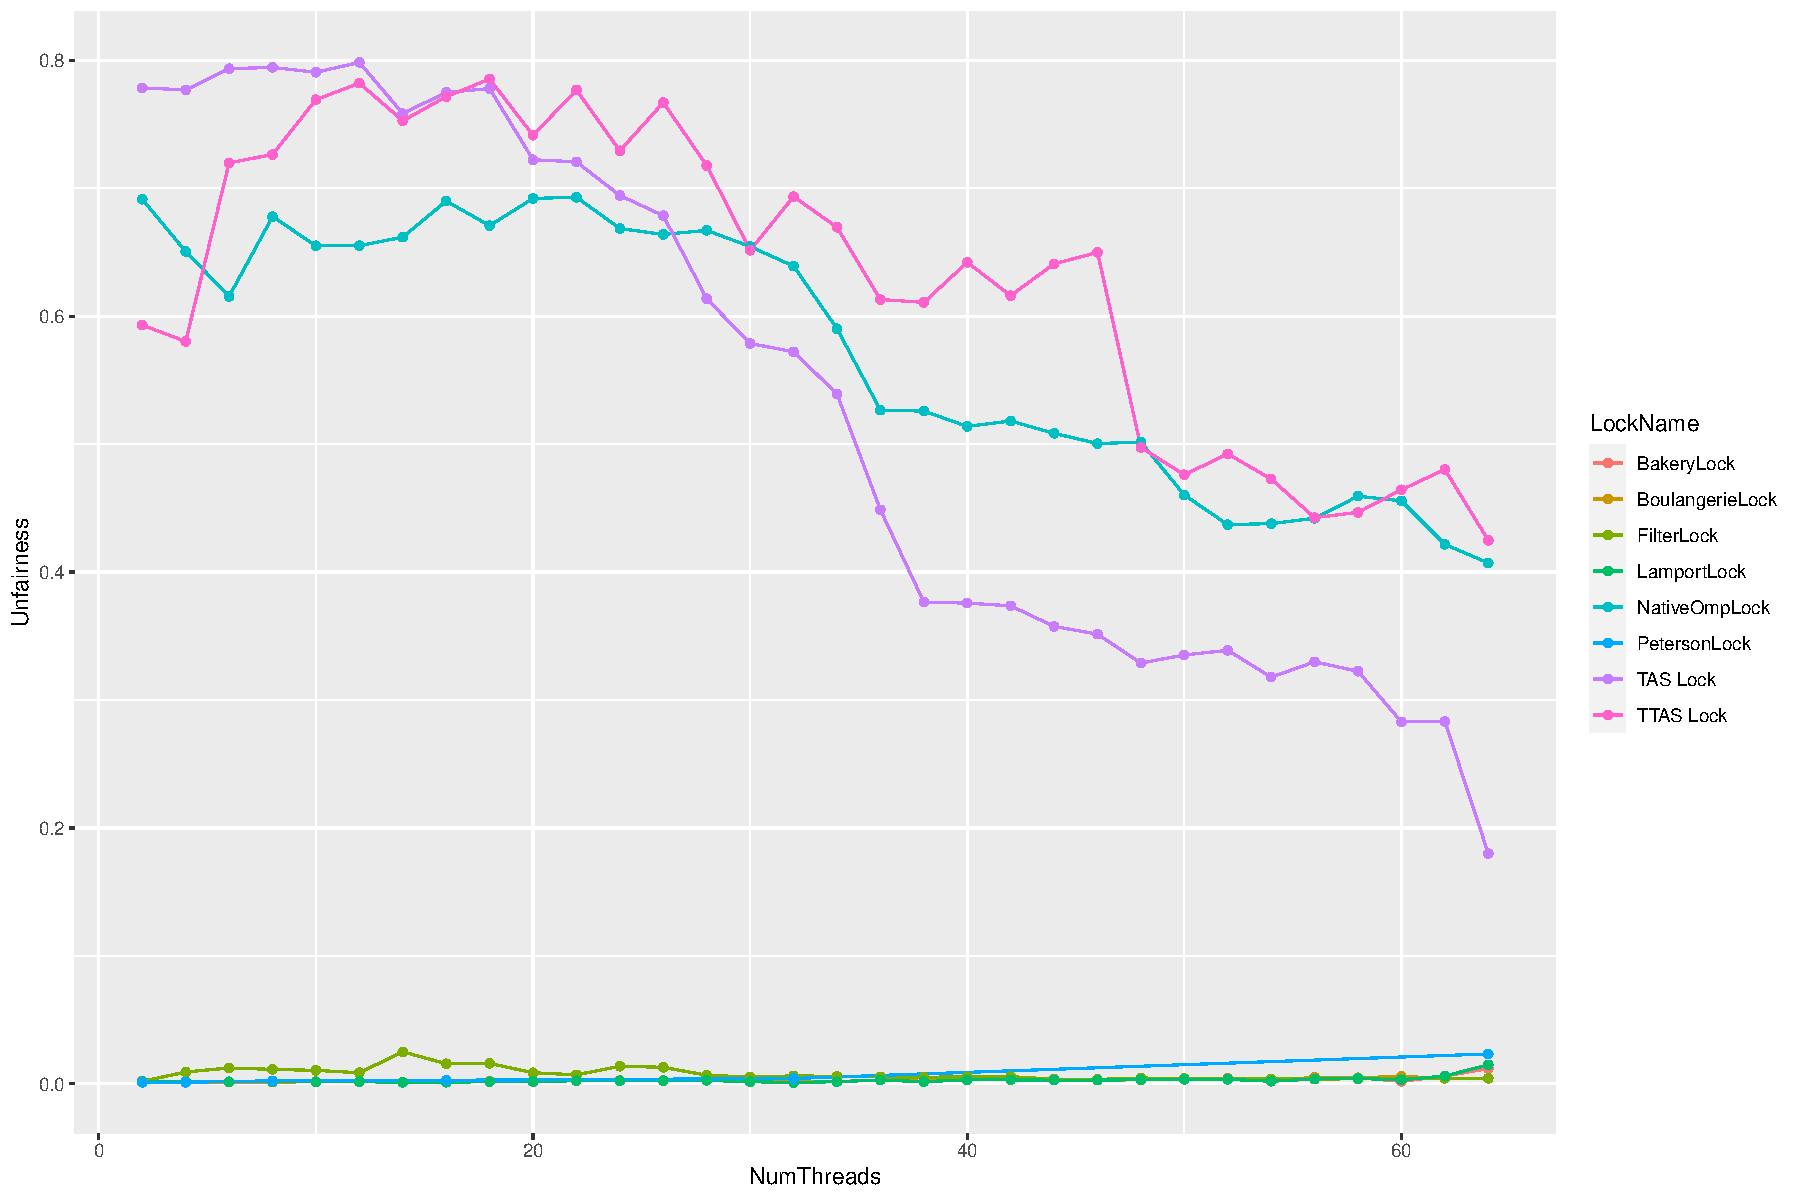
\includegraphics[width=\textwidth]{fig/fairness_all}
  \caption{Fairness for all implemented locks}
  \label{fig:fairness-all}
\end{figure}

\begin{figure}[H]
  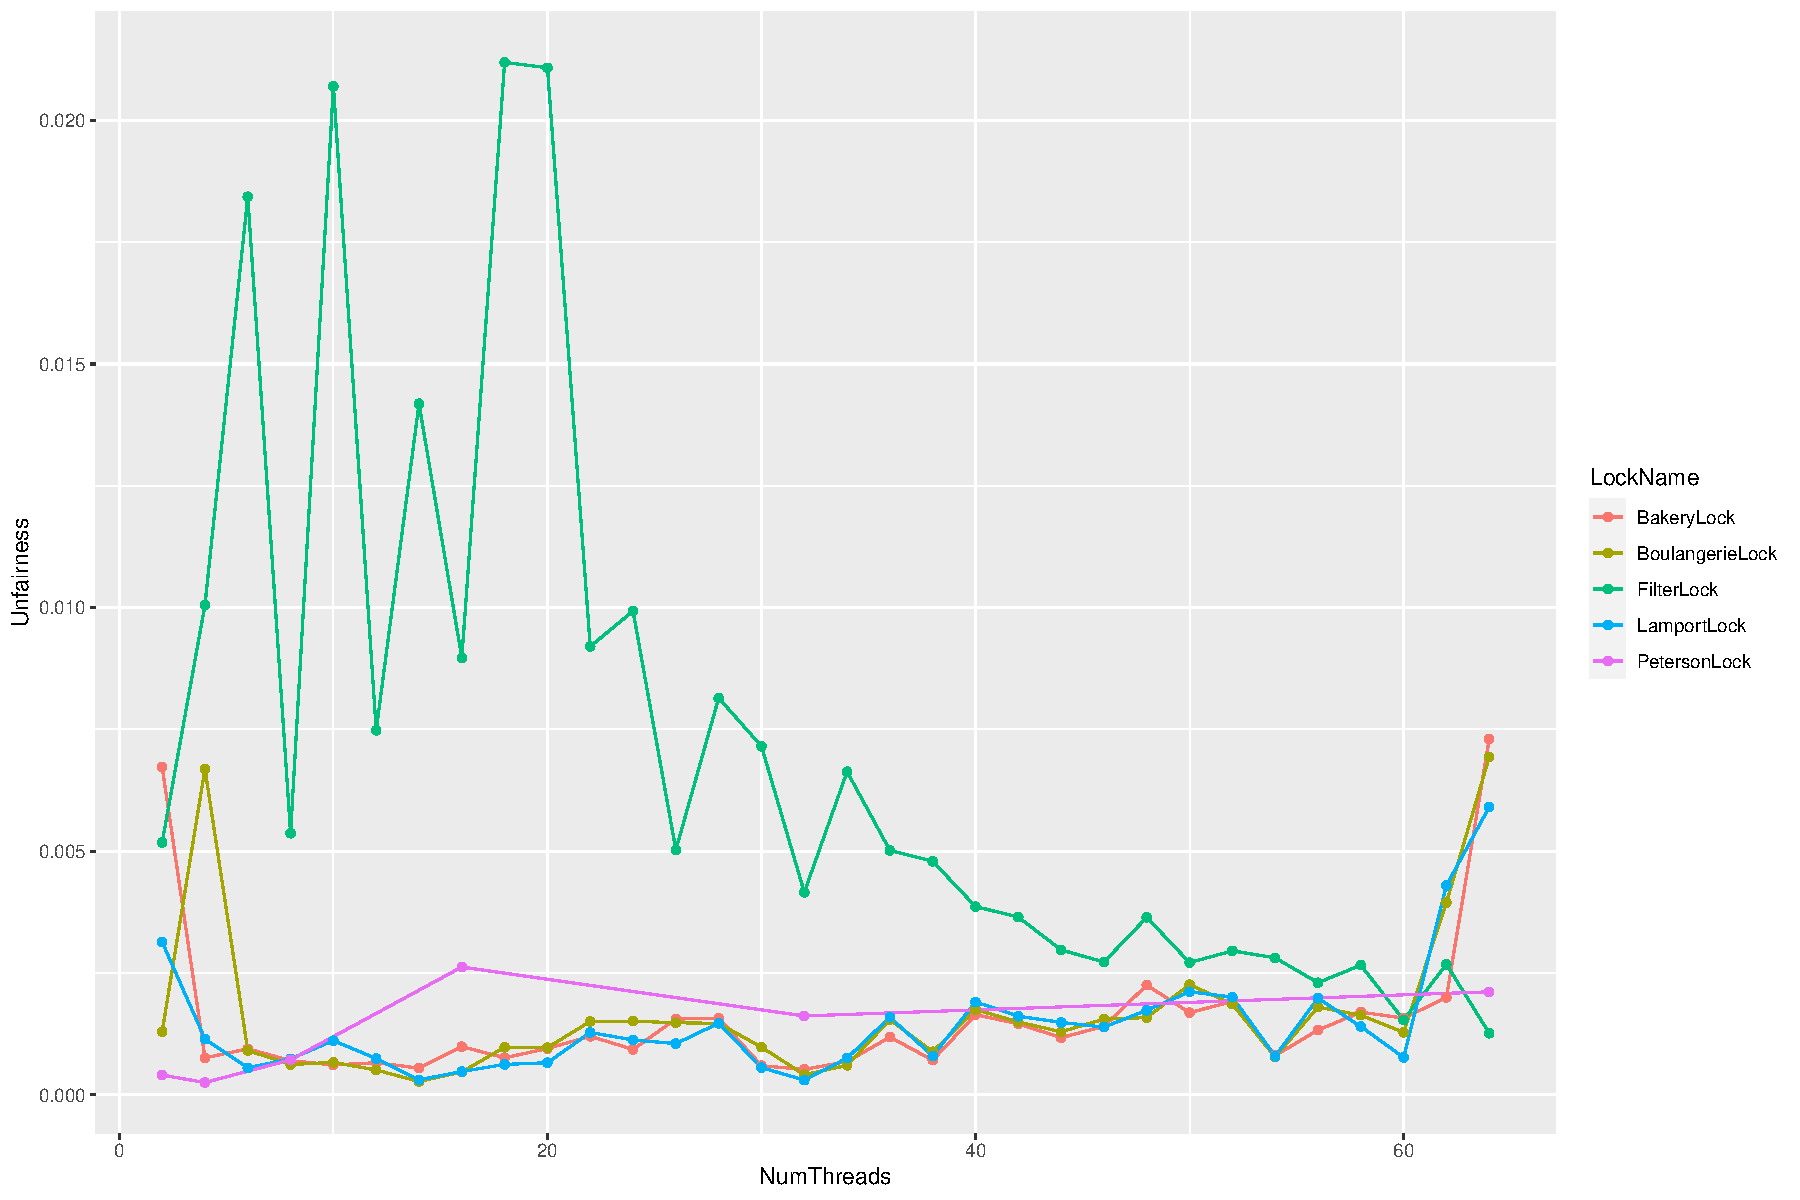
\includegraphics[width=\textwidth]{fig/fairness_no_tas}
  \caption{Fairness for custom locks}
  \label{fig:fairness-no-tas}
\end{figure}


\section{Performance}
In order to measure the performance of the locks we measure the time to acquire
$m = 1024$ locks in a row from $n$ number of threads.
Every acquisition loop is repeated 128 times, to ensure that CPU scheduling is not
biasing our data.
Finally, we repeat this procedure for increasing sizes in every lock, for a total
of slightly over 30 million lock acquisitions.

In order to determine these thresholds we ran the algorithm on various sizes and
settled with the first one where no more significative oscillation happened,
in order to remain in the 5 minutes limit imposed on the Nebula backend.

A further parameter we explored is the size of the critical section.
In all the iterations this is a fixed parameter, where we perform 2, 16, 128,
and 1024 while iterations, to emulate a load that un-trivializes the CS.

Finally, to evaluate the data we collected the time of each acquisition loop in
a CSV with the lock type and size.
We then computed for each lock a $5\%$-trimmed mean\footnote{$\alpha$-trimmed
mean is defined as a compromise between a median and a mean, where we discard
the $\alpha$ portion of the outer values then compute the sample mean on the
remaining ones.}, a robust estimator of the
central tendency.
Due to CPU scheduling in each execution we obtained some outliers that rendered
the data inconsistent.
Using the this robust estimator and collecting a lot of data a very stable
result across runs is ensured: by running the program again, the plots will vary
just slightly, but the main features analysed will persist.

We opted for this measure because it is almost identical to the latency: our
preliminary studies revealed that the behaviour of the $m$ iterations corresponds
to the single lock acquisition time.
This also corresponds to the theory, since the average time to lock is computed
using the sum of the individual lock times, that is the total lock time divided
by $m$.
Therefore, we obtained two plots scaled by a factor $m$.

Furthermore, this measure is the inverse of throughput, therefore sums up the
performance very coincisely.

In figure \ref{fig:meantime-2-all} we can observe the performance for all locks,
given CS size 2.
In particular the Filter lock will have a consistently much lower performance
regardless of the CS size, and will be therefore excluded from the follwing
plots in order to make the data readable.

\begin{figure}[H]
  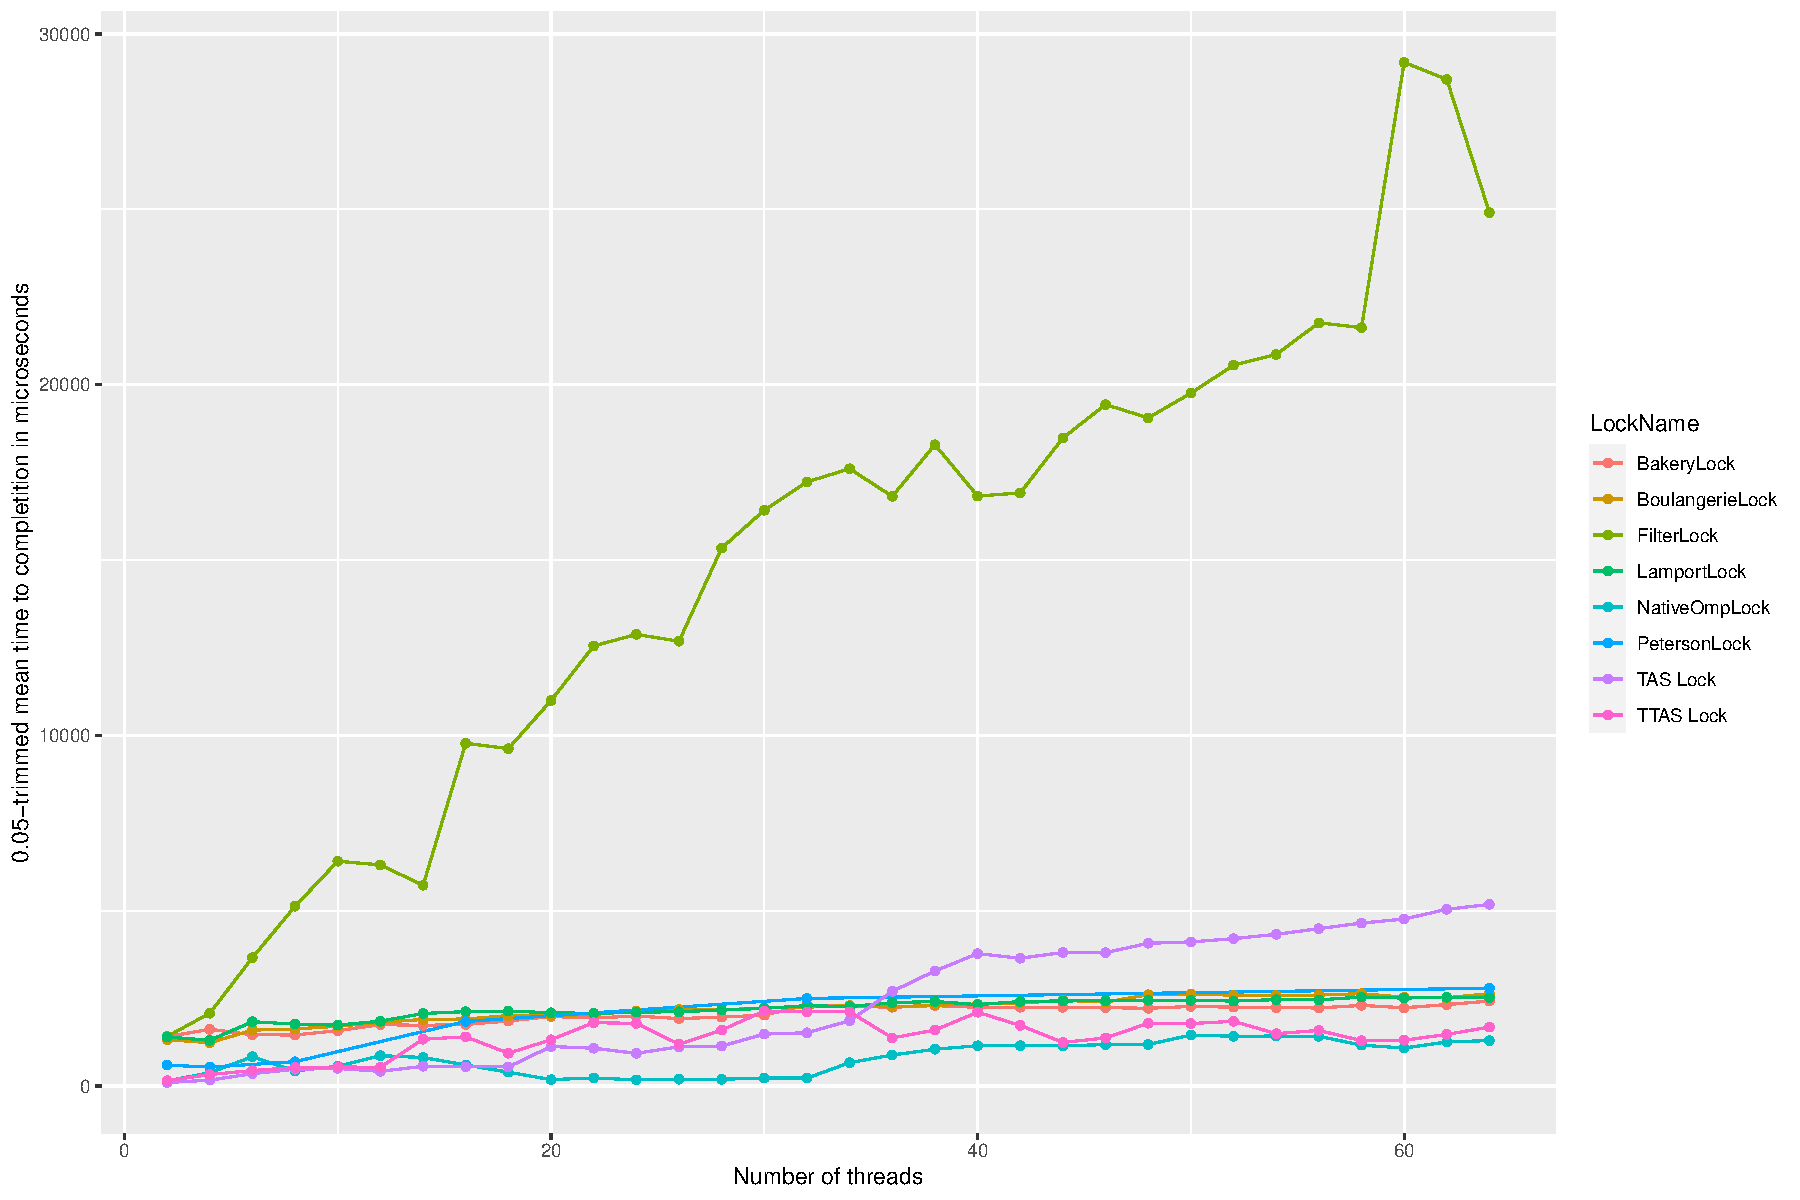
\includegraphics[width=\textwidth]{fig/meantime_2_all}
  \caption{$5\%$-trimmed mean of exec. time of all locks for CS load 2}
  \label{fig:meantime-2-all}
\end{figure}

The other locks, see figure \ref{fig:meantime-2-no-filter} are instead in a similar
range of performance, with the native OpenMP lock and TTAS leading, that maximise
performance at the expense of fairness.
The TAS lock is performant for lower amount of threads, but high contention will
make it the worst lock (except the Filter Lock).
Bakery, Lamport and Boulangerie all behave similarly, with a slow increase in
latency with increasing number of thread, but in a smooth way.
Finally, the peterson lock offers a very good performance for small locks, i.e.
up to size 8, being also quite fair.
\begin{figure}[H]
  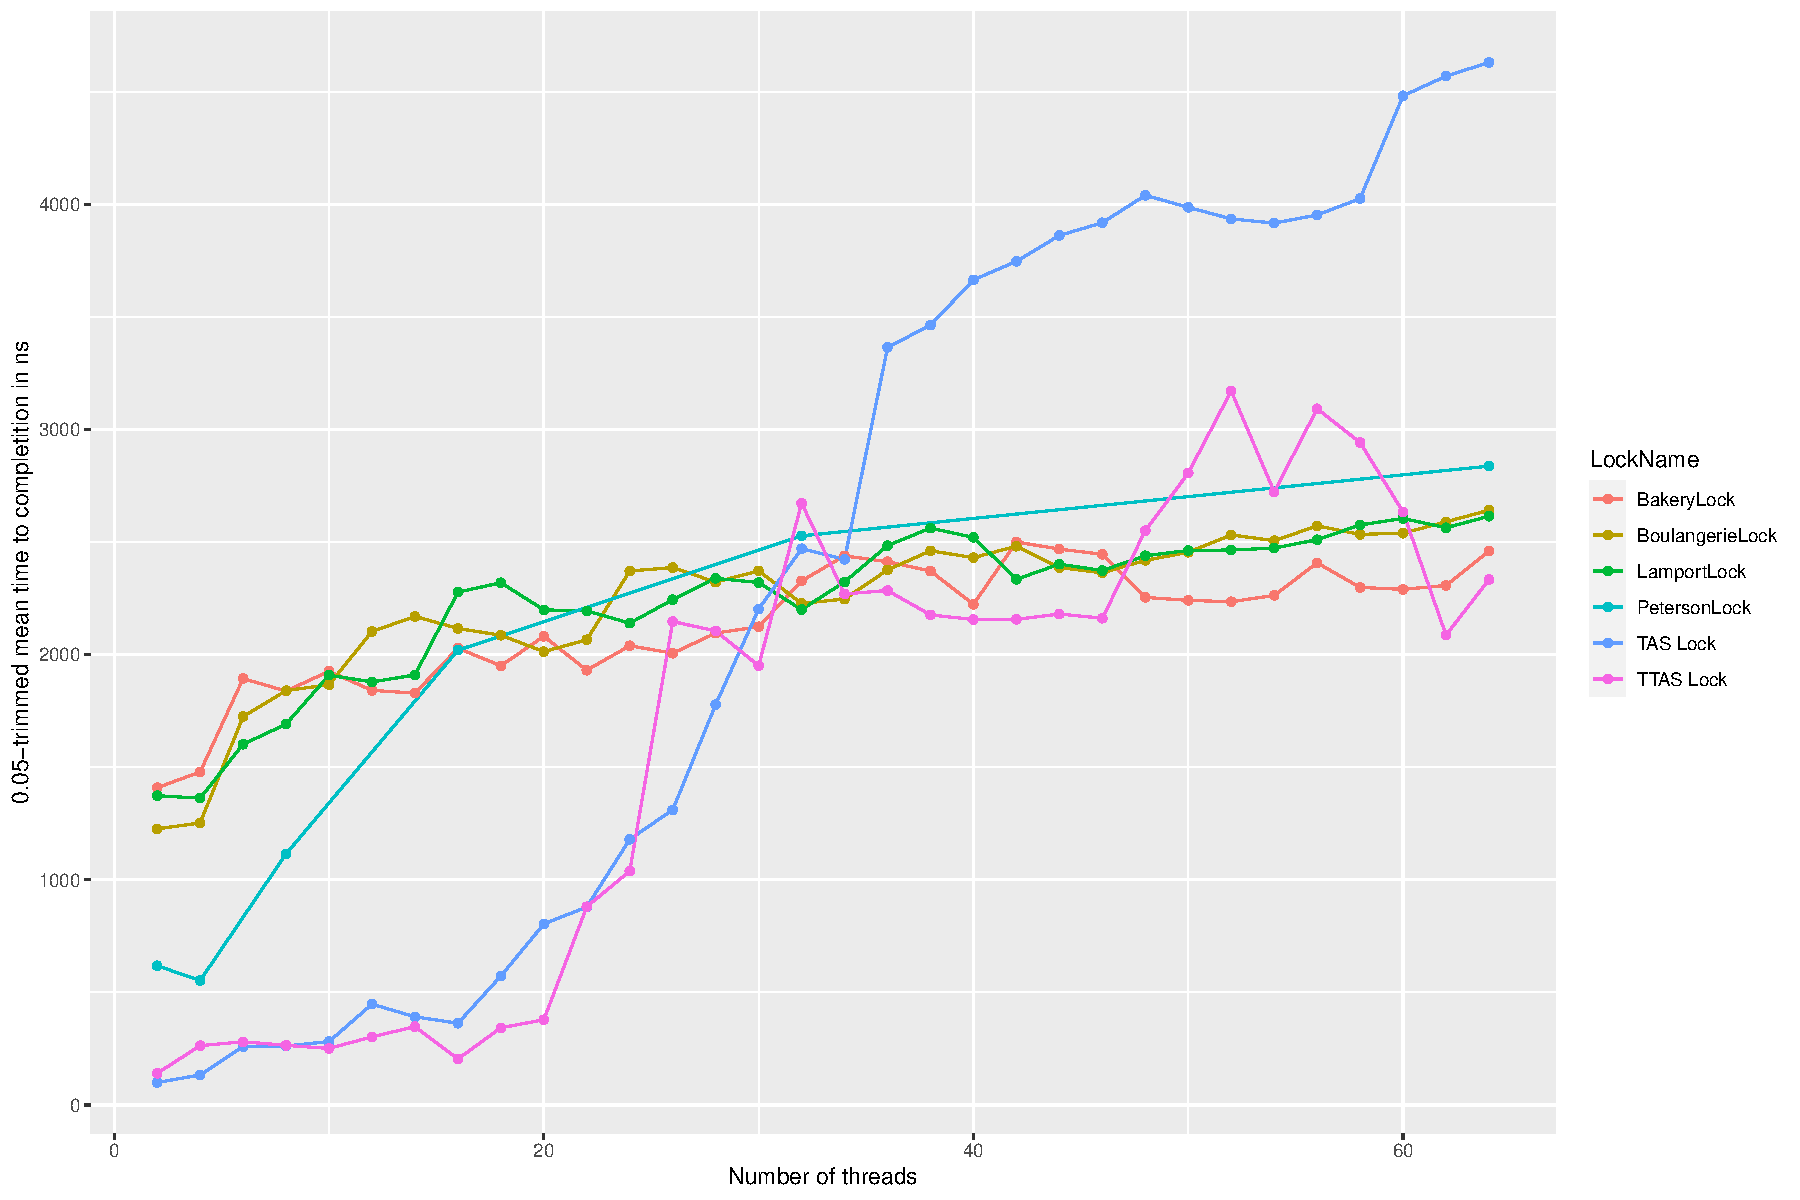
\includegraphics[width=\textwidth]{fig/meantime_2_no_filter}
  \caption{$5\%$-trimmed mean of exec. time of all but Filter lock for CS load 2}
  \label{fig:meantime-2-no-filter}
\end{figure}

We now introduce some load in the CS with parameters with CS size 128 (figure
\ref{fig:meantime-128-no-filter}) and 1024 (figure \ref{fig:meantime-1024-no-filter}).
It is apparent how the TAS lock performs poorly for the high contention
and that the native OpenMP lock consistently performs best, alongside the TTAS.

The Peterson Lock retains its behaviour, with a smooth log-like increase in latency
and the Bakery-based algorithm all perform as a cluster.
It is interesting to notice that the Boulangerie, that should be an improvement
over the Lamport Lock is almost in all cases performing slightly worse.
It can be that on this instruction set (x86\_64) the extra local computation is
actually worsening the algorithm.
The lock was implemented sticking strictly to the paper.

\begin{figure}[H]
  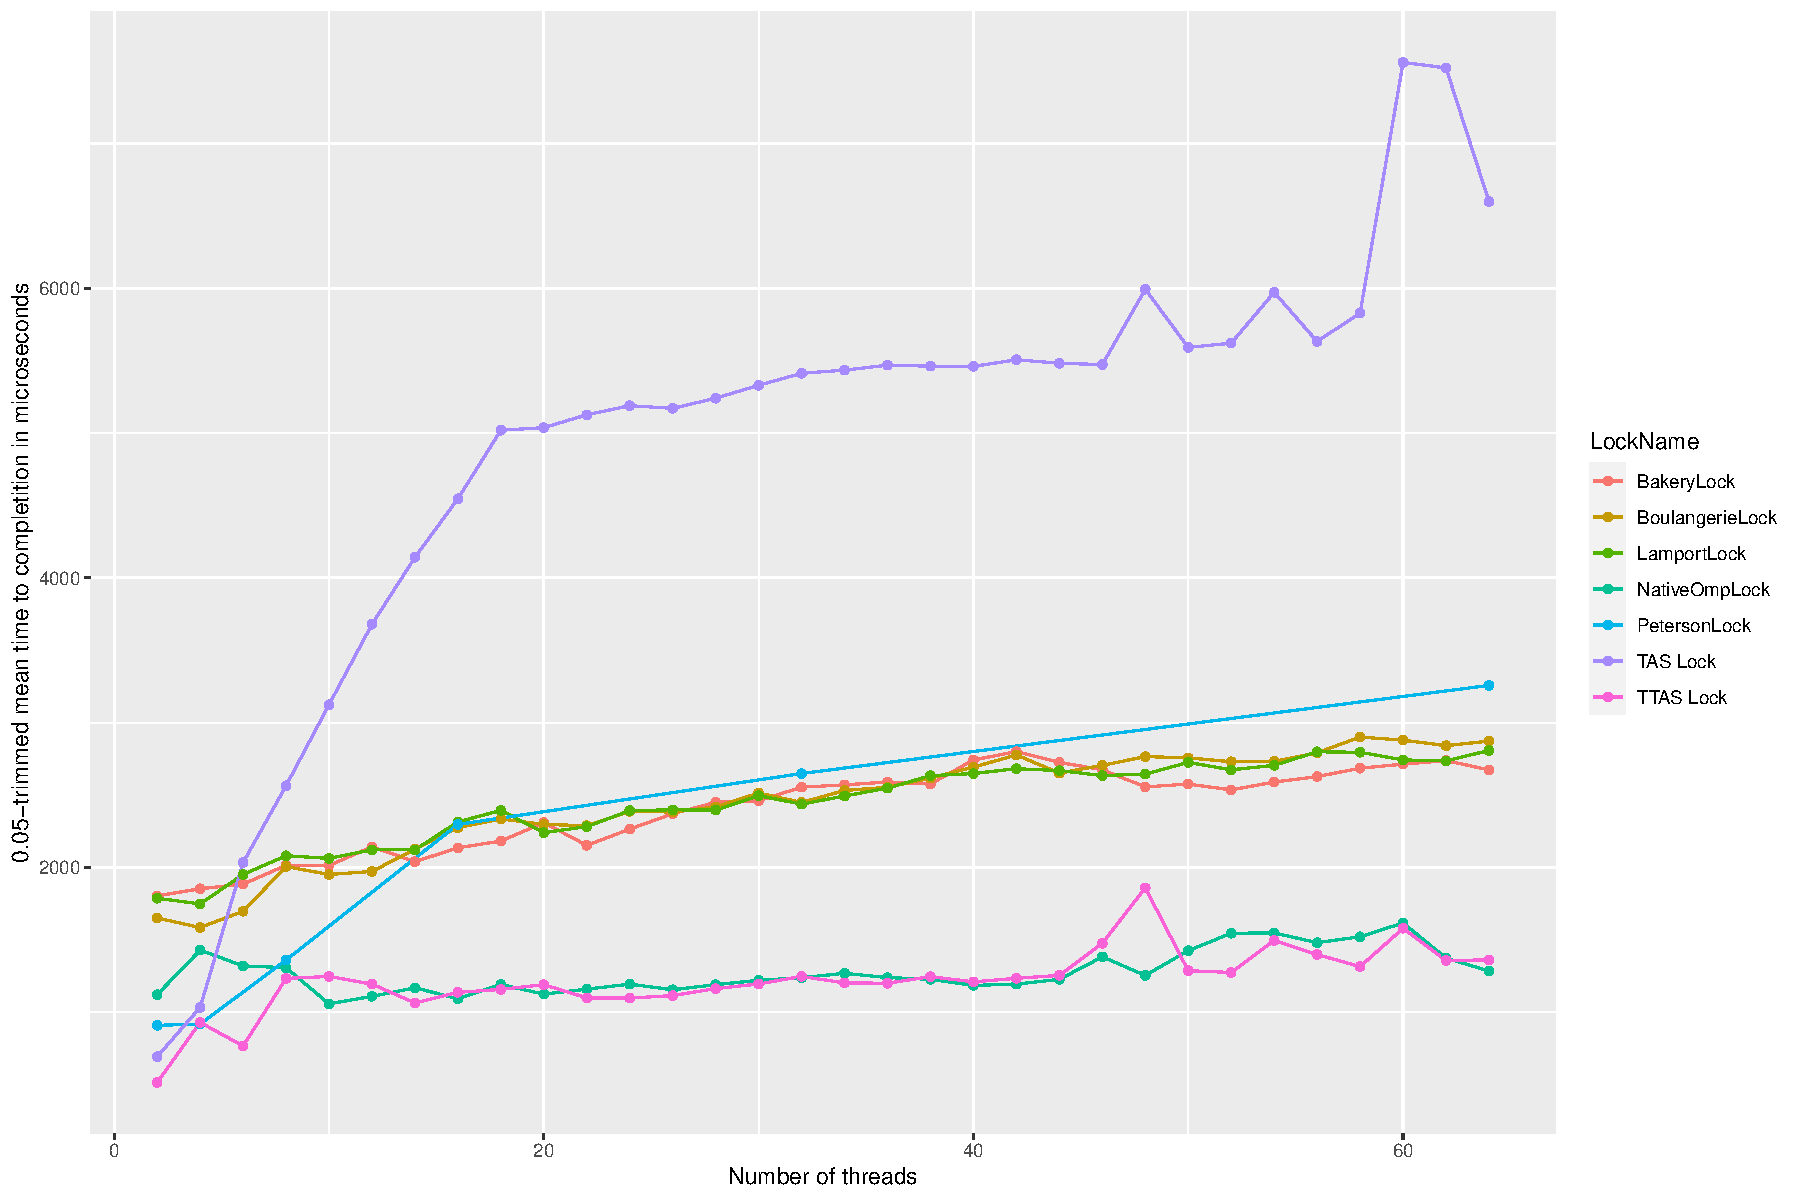
\includegraphics[width=\textwidth]{fig/meantime_128_no_filter}
  \caption{$5\%$-trimmed mean of exec. time of all but Filter lock for CS load 128}
  \label{fig:meantime-128-no-filter}
\end{figure}

\begin{figure}[H]
  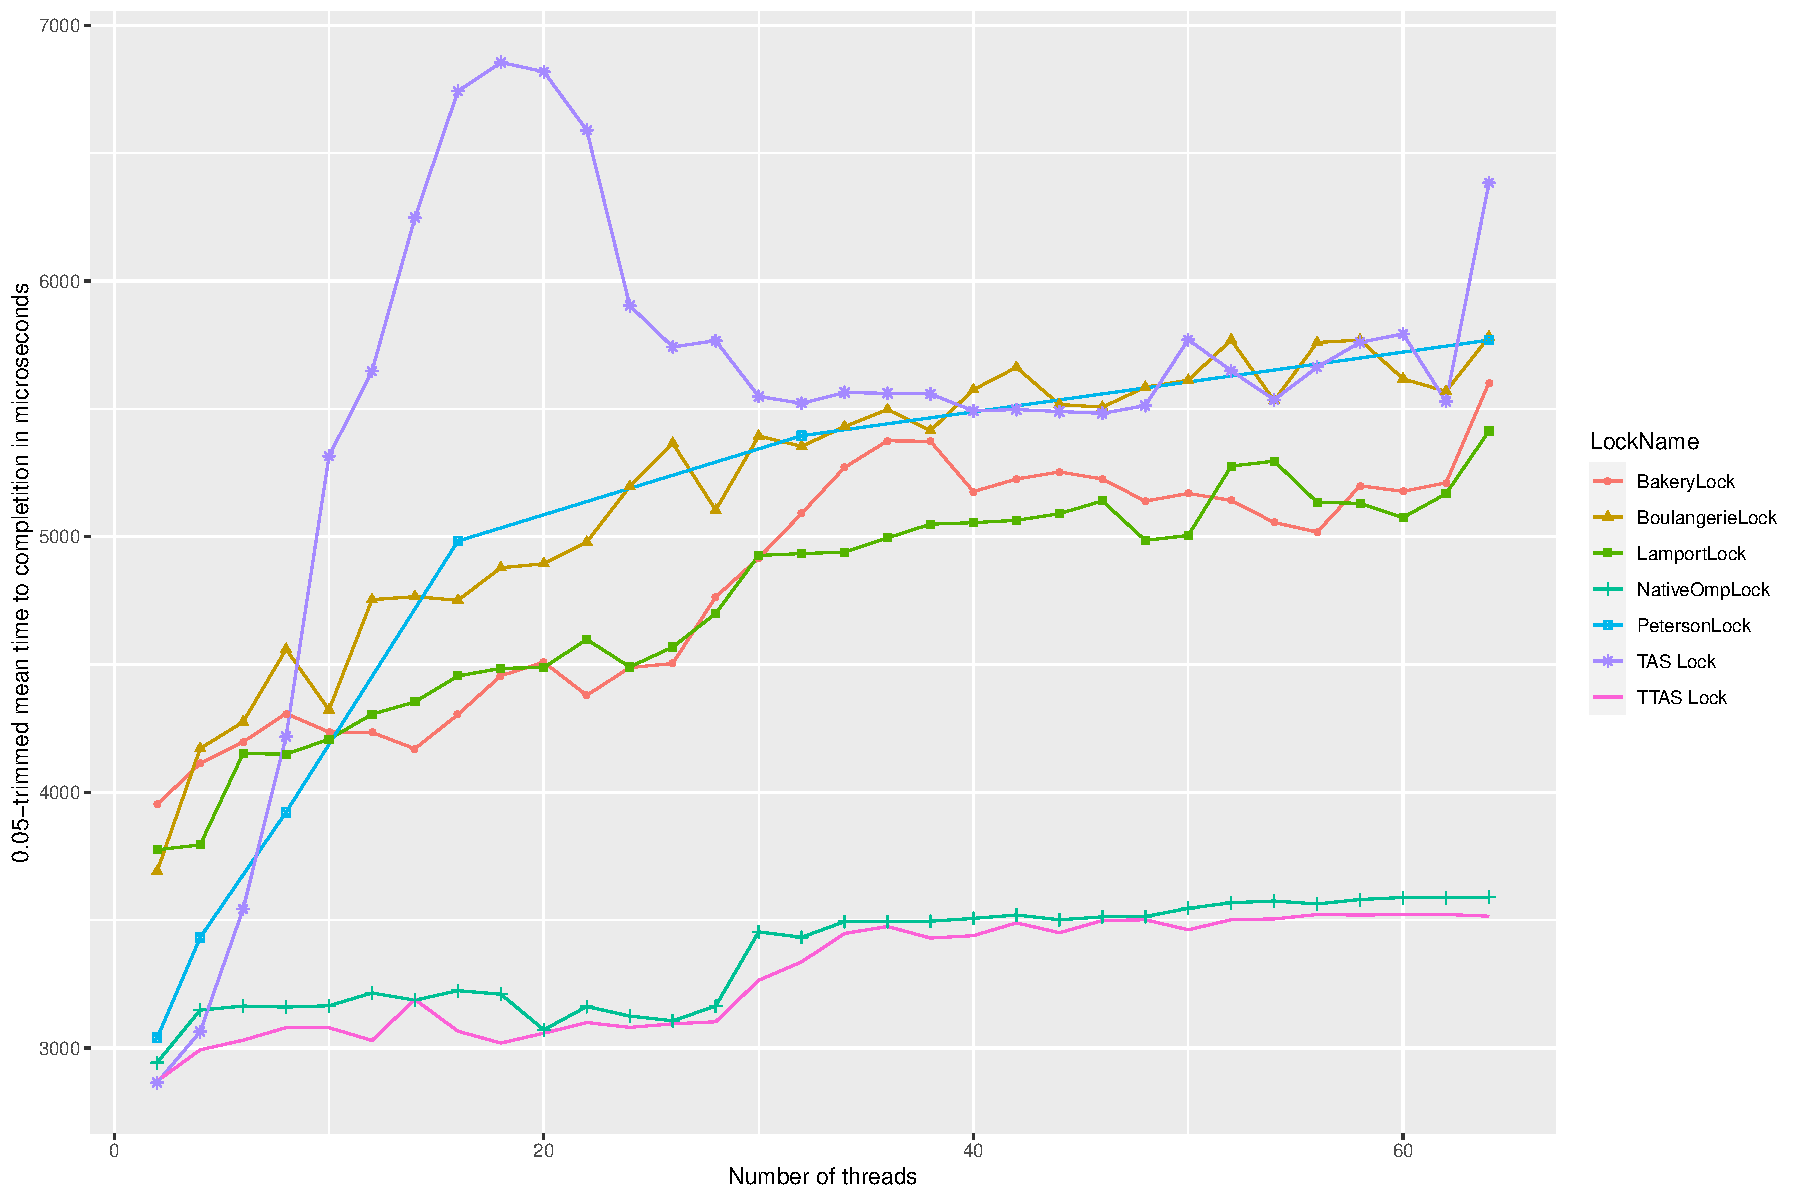
\includegraphics[width=\textwidth]{fig/meantime_1024_no_filter}
  \caption{$5\%$-trimmed mean of exec. time of all but Filter lock for CS load 1024}
  \label{fig:meantime-1024-no-filter}
\end{figure}


\printbibliography

\end{document}
